\documentclass{article}
\usepackage{graphicx}
\usepackage{amsmath}
\usepackage{pgfplots}
\usepackage{physics}
\usepackage{cancel}
\usepackage{enumitem}
\usepackage{txfonts}

\pgfplotsset{compat=1.18}

\newcommand{\Eth}{E_{\text{th}}}

\usepackage[a4paper, top=1cm, bottom=2cm, left=2cm, right=2cm, includehead, includefoot]{geometry}

\begin{document}

\noindent
Physics 4A - Classical Mechanics \hfill Prof. Roger King

\noindent\rule{\textwidth}{0.4pt}

\begin{center}
    \textbf{\LARGE Homework 14} \\
    \vspace{12pt}
    \large Aaron W. Tarajos \\
    \textit{\today}
\end{center}

\noindent\rule{\textwidth}{0.4pt}

\section*{Problem 1}
A wheel, whose moment of inertia is 0.0300 kg$\cdot$m$^2$, is accelerated from rest to 20.0 rad/s in 5.00 s. When the
external torque is removed, the wheel stops in 1 min. Find: (a) the frictional torque; (b) the external torque.

\subsection*{Solution}
\subsubsection*{Part a:}
Given the initial and final velocity we solve for the angular acceleration;
\[
	\alpha = \frac{\omega - \omega_0}{t} = \frac{0-20}{60} = \frac{1}{3}\ \text{rad}/\text{s}^2
\]
and then using Newton's second law we have;
\[
	\tau_k = I \alpha = 0.0300 \cdot \frac{1}{3} = \boxed{0.010} \text{N} \cdot \text{m}
\]
\subsubsection*{Part b:}
Similar to part a:

\[
	\alpha = \frac{\omega - \omega_0}{t} = \frac{20 - 0}{5} = 4\ \text{rad}/\text{s}^2
\]
then

\[
	\tau = I \alpha = 0.030 \cdot 4 = \boxed{0.12\ \text{N} \cdot \text{m}}
\]

\section*{Problem 2}
A block of mass m = 2.00 kg hangs vertically from a frictionless pulley of mass $M = 4.00$ kg and radius $R =
15.0$ cm. Find: (a) the acceleration of the block; (b) the tension in the rope; (c) the speed of the block after it has
fallen 40.0 cm-- assuming it started at rest. Treat the pulley as a solid disk.

\subsection*{Solution}


\section*{Problem 3}
A block of mass m = 2.00 kg can slide down a frictionless 53$^\circ$ incline, but it is connected to a pulley
of mass $M = 4.00$ kg and radius $R = 0.500$ m, as shown in the figure below. The pulley can be treated as
a disk. Find: (a) the angular acceleration of the pulley; (b) the speed of the block after it has slid 1.00 m,
starting from rest.

\begin{figure}[ht]
    \centering
    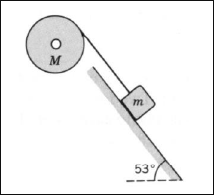
\includegraphics[scale=0.6]{drawing-1.png}
\end{figure}

\section*{Problem 4}
A car is traveling at 75.0 km/h has tires of 70.0 cm diameter. (a) What is the angular velocity of the tires about
their axles? (b) If the car is brought to a stop uniformly in 30.0 complete turns of the tires (without skidding),
what is the magnitude of the angular acceleration of the wheels? (c) How far does the car move during the
braking?

\section*{Problem 5}
The graph below shows the speed v versus time t for a 0.500 kg object of radius 6.50 cm that rolls smoothly
down a 30$^\circ$ ramp. The scale on the velocity axis is set by $v_s = 4.0$ m/s. What is the rotational inertia of the object?

\begin{figure}[ht]
    \centering
    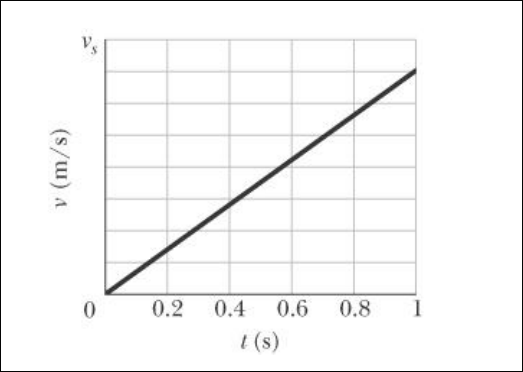
\includegraphics[scale=0.4]{drawing-2.png}
\end{figure}

\section*{Problem 6}
A hollow sphere of radius 0.15 m, with rotational inertia $I = 0.040$ kg$\cdot$m$^2$ about a line through its center of
mass, rolls without slipping up a surface inclined at 30° to the horizontal. At a certain initial position, the sphere’s
total kinetic energy is 20 J. (a) How much of this initial kinetic energy is rotational? (b) What is the speed of the
center of mass of the sphere at the initial position? When the sphere has moved 1.0 m up the incline from its
initial position, what are (c) its total kinetic energy and (d) the speed of its center of mass?

\section*{Problem 7}
A yo-yo has a rotational inertia of 900 g$\cdot$cm$^2$ and a mass of 100 g. Its axle radius is 3.2 mm, and its string is
120 cm long. The yo-yo rolls from rest down to the end of the string. (a) What is the magnitude of its linear
acceleration? (b) How long does it take to reach the end of the string? As it reaches the end of the string, what are
its (c) linear speed, (d) translational kinetic energy, (e) rotational kinetic energy, and (f) angular speed?

\section*{Problem 8}
A uniform rod is held vertically by two strings of negligible mass, as shown below. (a) Immediately after the
string is cut, what is the linear acceleration of the free end of the stick? (b) Of the middle of the stick?

\begin{figure}[ht]
    \centering
    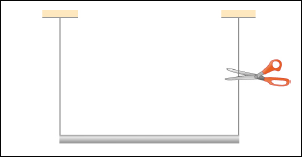
\includegraphics[scale=0.6]{drawing-3.png}
\end{figure}

\end{document}
